\documentclass[10pt,a4paper,oneside]{article}
\usepackage[utf8]{inputenc}
\usepackage{amsmath}
\usepackage{amsfonts}
\usepackage{amssymb}
\usepackage{graphicx}
\usepackage{breqn}
\usepackage{tikz} % system block diagram
\usepackage{textcomp}
\usetikzlibrary{shapes,arrows} % system block diagram
\usepackage{booktabs}
\usepackage[framed,numbered,autolinebreaks,useliterate]{mcode} % matlab code block
\author{Yangang Cao}
\date{February 15, 2019}
\newcommand{\degree}{^\circ}
\tikzset{
	delay/.style    = {draw, thick, rectangle, minimum height = 3em,
		minimum width = 3em},
	sum/.style      = {draw, circle, node distance = 2cm}, 
	prod/.style     = {draw, circle, node distance = 2cm},
	input/.style    = {coordinate}, % Input
	output/.style  = {coordinate} % Output
}
% Defining string as labels of certain blocks.
\newcommand{\product}{$\displaystyle \times$}
\newcommand{\delay}{\large$z^{-1}$}
\begin{document}

\title{Second-Order Bandpass/Bandreject Filter Design}
\maketitle 

The signal can be seen as a set of partials having different frenquencies and amplitudes. The filter can modify the amplitude of partials according to their frenquency.

\section{Definition of Bandpass/Bandreject Filters}

The two types of filters can be defined according to the following classification:

\begin{itemize}
	\item {\bfseries Bandpass (BP)} filters select frenquencies between a lower cut-off frenquency $f_{cl}$ and a higher cut-off frenquency $f_{ch}$. Frenquencies below $f_{cl}$ and frenquencies higher than $f_{ch}$ are attenuated.
	\item {\bfseries Bandreject (BR)} filters attenuate frenquencies between a lower cut-off frenquency $f_{cl}$ and a higher cut-off frenquency $f_{ch}$. Frenquencies below $f_{cl}$ and frenquencies higher than $f_{ch}$ are passed.
\end{itemize}

The bandpass can produce effects such as the imitation of a telephone line or of a mute on an acoustical instrument; the bandreject can divide the audible spectrum into two bands that seem to be uncorrelated.

\section{Canonical Form}
There are various ways to implement a filter, the simplest being the canonical filter, as shown in following figure for a second-order filter, which can be implemented by the defference equations
\[
x_h(n) = x(n) - a_1x_h(n-1) - a_2x_h(n-2)
\]
\[
y(n) = b_0x_h(n) + b_1x_h(n-1) + b_2x_h(n-2),
\]



\begin{center}
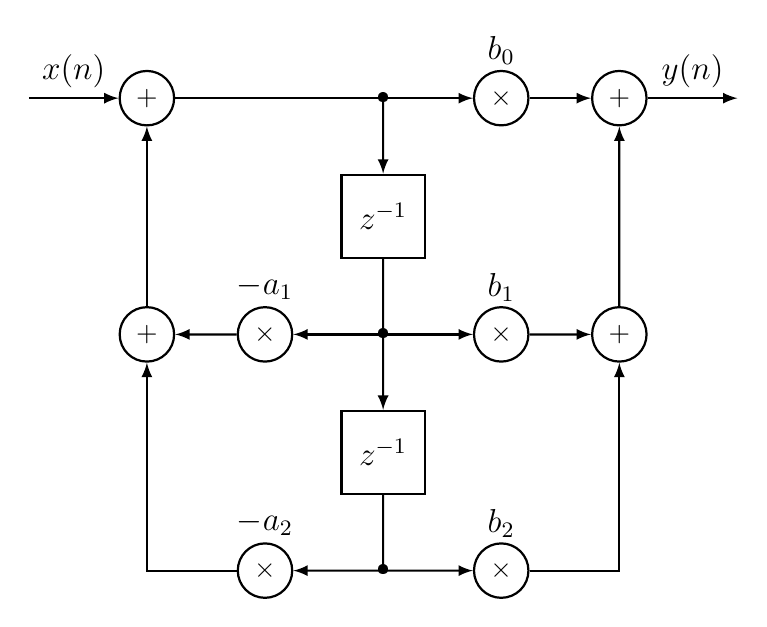
\begin{tikzpicture}[auto, thick, node distance=0.6cm, >=latex, scale = 0.75]
\draw
% Drawing the blocks of first filter 
node at (0,0)[sum] (s1) {$+$}
node at (6,0)[prod] (p1) {\product} node[above of = p1] {\large$b_0$}
node at (8,0)[sum] (s2) {$+$}
node at (4,-2) [delay] (d1) {\delay}
node at (0,-4) [sum] (s3) {$+$}
node at (2,-4) [prod] (p2) {\product} node[above of = p2] {\large$-a_1$}
node at (6,-4) [prod] (p3) {\product} node[above of = p3] {\large$b_1$}
node at (8,-4) [sum] (s4) {$+$}
node at (4,-6) [delay] (d2) {\delay}
node at (2,-8) [prod] (p4) {\product} node[above of = p4] {\large$-a_2$}
node at (6,-8) [prod] (p5) {\product} node[above of = p5] {\large$b_2$};

\draw[->](-2,0) -- node {\large$x(n)$}(s1);
\draw[->](s1) -- node {} (p1);
\draw[->](p1) -- node {} (s2);
\draw[->](s2) -- node {\large$y(n)$} (10,0);
\draw[->](4,0) -- node {} (d1);
\draw[->](d1) -- node {} (d2);
\draw[<->](p2) -- node {} (p3);
\draw[->](p2) -- node {} (s3);
\draw[->](s3) -- node {} (s1);
\draw[->](p3) -- node {} (s4);
\draw[->](s4) -- node {} (s2);
\draw[-](d2) -- node {} (4,-8);
\draw[<->](p4) -- node {} (p5);
\draw[->](p4) -| node {} (s3);
\draw[->](p5) -| node {} (s4);

\draw
node at (4,0) {\textbullet} 
node at (4,-4){\textbullet}
node at (4,-8){\textbullet};
\end{tikzpicture}
\end{center}
and leads to the transfer function by setting $a_2 = b_2 = 0$, this reduces to a first-order filter which, can be used to implement an allpass, lowpass or highpass with the coefficients of following table
\begin{center}
	\begin{tabular}{cccc}
	\toprule  %添加表格头部粗线
	 & {$b_0$}&{$b_1$}&{$a_1$}\\
	\midrule  %添加表格中横线
	Lowpass&K/(K+1)& K/(K+1) & (K-1)/(K+1)\\
	Highpass& 1/(K+1)& -1/(K+1) & (K-1)/(K+1)\\
	Allpass&(K-1)/(K+1)&1&(K-1)/(K+1)\\
	\bottomrule %添加表格底部粗线
	\end{tabular}
\end{center}
where $K$ depends on the cut-off frequency $f_c$ by
\[
K=\tan(\pi f_c/f_S).
\]



\section{Second-Order Allpass-Based Filter}
The implementation of tunable bandpass and bandreject filters can be achieved with a second-order allpass filter. The transfer function of a second-order allpass filter is given by
\[
A(z) = \frac{-c + d(1-c)z^{-1} + z^{-2}}{1 + d(1-c)z^{-1} - cz^{-2}}
\]
\[
c = \frac{\tan(\pi f_b/f_S) - 1}{\tan(\pi f_b/f_S) + 1}
\]
\[
d = -\cos(2\pi f_c/f_S),
\]
with the corresponding difference equatons
\[
x_h(n) = x(n) - d(1-c)x_h(n-1) + cx_h(n-2)
\]
\[
y(n) = -cx_h(n) + d(1-c)x_h(n-1) + x_h(n-2).
\]
The parameter $d$ adjusts the center frequency and the parameter $c$ the bandwidth. The
magnitude response is again equal to one and the phase response approaches ${-360\degree}$ for high
frequencies. The cut-off frequency $f_c$ determines the point on the phase curve where the phase response passes ${-180\degree}$. The width or slope of the phase transition around the cut-off frequency is controlled by the bandwidth parameter $f_b$. The following block diagram shows the second-order allpass filter,
\begin{center}
	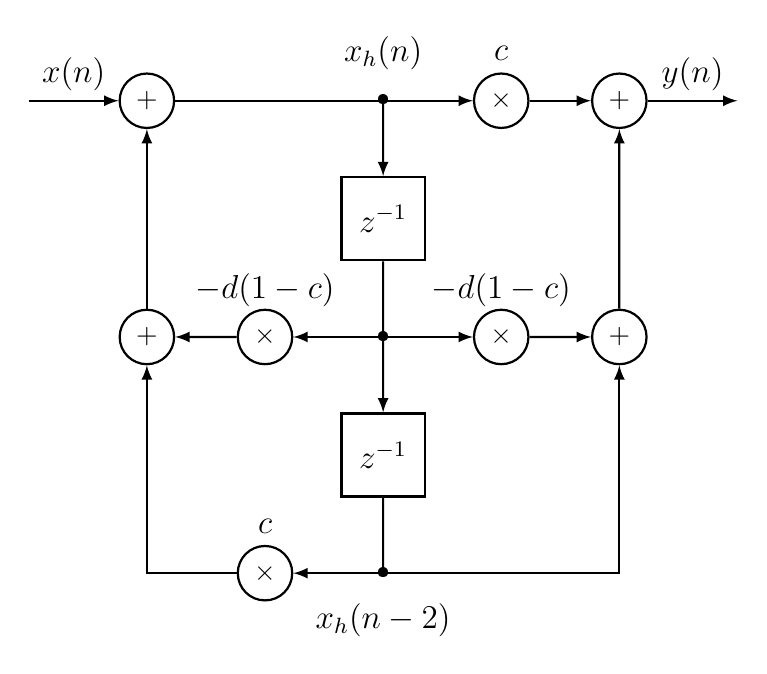
\begin{tikzpicture}[auto, thick, node distance=0.6cm, >=latex, scale = 0.75]
	\draw
	% Drawing the blocks of first filter 
	node at (0,0)[sum] (s1) {$+$}
	node at (6,0)[prod] (p1) {\product} node[above of = p1] {\large$c$}
	node at (8,0)[sum] (s2) {$+$}
	node at (4,-2) [delay] (d1) {\delay}
	node at (0,-4) [sum] (s3) {$+$}
	node at (2,-4) [prod] (p2) {\product} node[above of = p2] {\large$-d(1-c)$}
	node at (6,-4) [prod] (p3) {\product} node[above of = p3] {\large$-d(1-c)$}
	node at (8,-4) [sum] (s4) {$+$}
	node at (4,-6) [delay] (d2) {\delay}
	node at (2,-8) [prod] (p4) {\product} node[above of = p4] {\large$c$}
	 ;
	
	\draw[->](-2,0) -- node {\large$x(n)$}(s1);
	\draw[->](s1) -- node {} (p1);
	\draw[->](p1) -- node {} (s2);
	\draw[->](s2) -- node {\large$y(n)$} (10,0);
	\draw[->](4,0) -- node {} (d1);
	\draw[->](d1) -- node {} (d2);
	\draw[<->](p2) -- node {} (p3);
	\draw[->](p2) -- node {} (s3);
	\draw[->](s3) -- node {} (s1);
	\draw[->](p3) -- node {} (s4);
	\draw[->](s4) -- node {} (s2);
	\draw[-](d2) -- node {} (4,-8);
	\draw[<->](p4) -| node {} (s4);
	\draw[->](p4) -| node {} (s3);
	
	\draw
	node at (4,0)(n1) {\textbullet} node[above of = n1]{\large$x_h(n)$}
	node at (4,-4){\textbullet}
	node at (4,-8)(n2){\textbullet} node[below of = n2]{\large$x_h(n-2)$};
	\end{tikzpicture}
\end{center}
and corresponding state and output equations are:
\[
\begin{bmatrix}x_h(n)\\x_h(n-1)\end{bmatrix} = \begin{bmatrix}
-d(1-c)&c\\
1&0
\end{bmatrix}
\begin{bmatrix}x_h(n-1)\\x_h(n-2)\end{bmatrix} + \begin{bmatrix}1\\0\end{bmatrix}
x(n)\]
\[
y(n) = \begin{bmatrix}(1-c^2)d&1-c^2\end{bmatrix}
\begin{bmatrix}x_h(n-1)\\x_h(n-2)\end{bmatrix} + (-c)x(n).
\]

Actually, the state and output equations represent the same meaning as the difference equations, but difference in format. The difference equations are usually easy to comprehend, howere, state and output equations are more widely used in modern control theory, so we implement all kinds of filters by this format. The second-order allpass filter implementation can be obtained by the following {\bfseries Matlab} code.
\begin{lstlisting}
function y = secondallpass(audio, para)
% y = secondallpass(audio, para)
% Author: Yangang Cao
% Applies a allpass filter to the input signal.
% para(1) is the normalized center frequency in (0,1), i.e. 2*fc/fS.
% para(2) is the normalized bandwidth in (0,1) i.e. 2*fb/fS.
c = (tan(pi*para(2)/2)-1) / (tan(pi*para(2)/2)+1);
d = -cos(pi*para(1));
x = [0; 0];
x_1 = 0;
A = [-d*(1-c), c; 1, 0];
B = [1; 0];
C = [d*(1-c^2), 1-c^2];
D = -c;
for n=1:length(audio)
	x_1 = A * x + B * audio(n);
	y(n) = C * x + D * audio(n);
	x = x_1;
end
\end{lstlisting}
\section{Second-Order Bandpass/Bandreject Filter}
Second-order bandpass and bandreject filters can be described by the following transfer function
\[
H(z) = \frac{1}{2}[1 \mp A(z)]\quad(BP/BR-/+)
\]
\[
A(z) = \frac{-c + d(1-c)z^{-1} + z^{-2}}{1 + d(1-c)z^{-1} - cz^{-2}}
\]
\[
c = \frac{\tan(\pi f_b/f_S) - 1}{\tan(\pi f_b/f_S) + 1}
\]
\[
d = -\cos(2\pi f_c/f_S),
\]
where a tunable second-order allpass $A(z)$ with tuning parameters $c$ and $d$ is used. The minus sign (-) denotes the bandpass operation and the plus sign (+) the bandreject operation. The block diagram in following figure represents the operations involved in performing the bandpass/bandreject filtering.
\begin{center}
	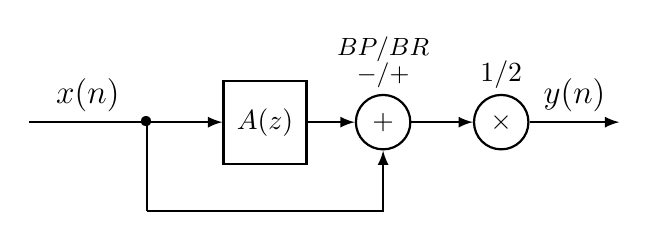
\begin{tikzpicture}[auto, thick, node distance=0.6cm, >=latex, scale = 0.75]
	\draw
	node at (2,0)[delay] (d1) {$A(z)$}
	node at (4,0)[sum] (s1) {$+$} 
	node[above of = s1]{\small$-/+$} node[above of=s1,above=1]{\small{$BP/BR$}}
	node at (6,0) [prod] (p1) {\product} node[above of = p1]{$1/2$};
	
	\draw[-](-2,0) -- node {\large$x(n)$}(0,0);
	\draw[->](0,0) -- node {} (d1);
	\draw[->](d1) -- node {} (s1);
	\draw[->](s1) -- node {} (p1);
	\draw[->](p1) -- node {\large$y(n)$} (8,0);
	\draw[-](0,0) -- node {} (0,-1.5);
	\draw[->](0,-1.5) -| node {} (s1);
	
	\draw
	node at (0,0) {\textbullet};
	\end{tikzpicture}
\end{center}

The difference equations of second-order bandpass filter are: 
\[
x_h(n) = x(n) - d(1-c)x_h(n-1) + cx_h(n-2)
\]
\[
y(n) = \frac{1+c}{2}x_h(n) - \frac{1+c}{2}x_h(n-2),
\]
and corresponding state and output equations are:
\[
\begin{bmatrix}x_h(n)\\x_h(n-1)\end{bmatrix} = \begin{bmatrix}
-d(1-c)&c\\
1&0
\end{bmatrix}
\begin{bmatrix}x_h(n-1)\\x_h(n-2)\end{bmatrix} + \begin{bmatrix}1\\0\end{bmatrix}
x(n)\]
\[
y(n) = \begin{bmatrix}\frac{d(c^2-1)}{2}&\frac{c^2-1}{2}\end{bmatrix}
\begin{bmatrix}x_h(n-1)\\x_h(n-2)\end{bmatrix} + \frac{1+c}{2}x(n)
\]
A second-order bandpass filter implementation can be obtained by the following {\bfseries Matlab} code.
\begin{lstlisting}
function y = apbandpass(audio, para)
% y = apbandpass(audio, para)
% Author: Yangang Cao
% Applies a bandpass filter to the input signal.
% para(1) is the normalized center frequency in (0,1), i.e. 2*fc/fS.
% para(2) is the normalized bandwidth in (0,1) i.e. 2*fb/fS.
c = (tan(pi*para(2)/2)-1) / (tan(pi*para(2)/2)+1);
d = -cos(pi*para(1));
x = [0; 0];
x_1 = 0;
A = [-d*(1-c), c; 1, 0];
B = [1; 0];
C = [d*(c^2-1)/2, (c^2-1)/2];
D = (1+c)/2;
for n=1:length(audio)
	x_1 = A * x + B * audio(n);
	y(n) = C * x + D * audio(n);
	x = x_1;
end
\end{lstlisting}

The difference equations of second-order bandreject filter are: 
\[
x_h(n) = x(n) - d(1-c)x_h(n-1) + cx_h(n-2)
\]
\[
y(n) = \frac{1-c}{2}x_h(n) + d(1-c)x_h(n-1) + \frac{1-c}{2}x_h(n-2),
\]
and corresponding state and output equations are:
\[
\begin{bmatrix}x_h(n)\\x_h(n-1)\end{bmatrix} = \begin{bmatrix}
-d(1-c)&c\\
1&0
\end{bmatrix}
\begin{bmatrix}x_h(n-1)\\x_h(n-2)\end{bmatrix} + \begin{bmatrix}1\\0\end{bmatrix}
x(n)\]
\[
y(n) = \begin{bmatrix}\frac{d(1-c^2)}{2}&\frac{1-c^2}{2}\end{bmatrix}
\begin{bmatrix}x_h(n-1)\\x_h(n-2)\end{bmatrix} + \frac{1-c}{2}x(n)
\]
A second-order bandreject filter implementation can be obtained by the following {\bfseries Matlab} code.
\begin{lstlisting}
function y = apbandreject(audio, para)
% y = apbandreject(audio, para)
% Author: Yangang Cao
% Applies a bandreject filter to the input signal.
% para(1) is the normalized center frequency in (0,1), i.e. 2*fc/fS.
% para(2) is the normalized bandwidth in (0,1) i.e. 2*fb/fS.
c = (tan(pi*para(2)/2)-1) / (tan(pi*para(2)/2)+1);
d = -cos(pi*para(1));
x = [0; 0];
x_1 = 0;
A = [-d*(1-c), c; 1, 0];
B = [1; 0];
C = [d*(1-c^2)/2, (1-c^2)/2];
D = (1-c)/2;
for n=1:length(audio)
	x_1 = A * x + B * audio(n);
	y(n) = C * x + D * audio(n);
	x = x_1;
end
\end{lstlisting}
\end{document}
